 
\chapter{Regression Models for Count Outcomes}
\label{chapter::count}
 
A random variable for counts can take values in $\left\{ 0,1,2,\ldots\right\} $. This type of variable is common in applied statistics. For example, it can represent how many times you visit the gym every week, how many lectures you have missed in the linear model course, how many traffic accidents happened in certain areas during certain periods, etc. This chapter focuses on statistical modeling of those outcomes given covariates. \citet{hilbe2014modeling} is a textbook focusing on count outcome regressions. 




\section{Some random variables for counts\label{sec:Some-random-variables-counts}}


I first review four canonical choices of random variables for modeling count data.

\subsection{Poisson}

A random variable $y$ is Poisson$(\lambda)$ if its probability mass
function is
\[
\pr(y=k)=e^{-\lambda}\frac{\lambda^{k}}{k!}, \quad(k=0,1,2,\ldots)
\]
which sums to $1$ by the Taylor expansion formula $e^{\lambda} =  \sum_{k=0}^{\infty}  \frac{\lambda^{k}}{k!}$.
The Poisson$(\lambda)$ random variable has the following properties:
\begin{proposition}
If $y\sim \textup{Poisson} (\lambda)$, then 
$
E(y)=\var(y)=\lambda.
$
\end{proposition}
%
%\begin{proposition}
%If $y_1\ind y_2$ with $y_{1}\sim$Poisson$(\lambda_{1})$ and $y_{2}\sim$Poisson$(\lambda_{2})$,
%then
%\[
%\begin{array}{ccc}
%y_{1}+y_{2} & \sim & \textup{Poisson}(\lambda_{1}+\lambda_{2}),\\
%y_{1}\mid y_{1}+y_{2} = n & \sim & \textup{Binomial}\left(n, \frac{\lambda_{1}}{\lambda_{1}+\lambda_{2}}\right).
%\end{array}
%\]
% 
%\end{proposition}
\begin{proposition}
If $y_1, \ldots,  y_K$ are mutually independent with $y_k\sim \textup{Poisson}(\lambda_k)$ for $k=1,\ldots, K$,
then
$$
y_{1}+\cdots + y_{K}  
\sim  \textup{Poisson}(\lambda),
$$
and
$$
(y_{1}, \ldots, y_K) \mid y_{1}+ \cdots + y_{K} = n  
\sim  \textup{Multinomial}\left(n,  (\lambda_1/ \lambda, \ldots, \lambda_K / \lambda ) \right),
$$ 
where $\lambda = \lambda_{1}+ \cdots + \lambda_{K}$. 

Conversely, if $S\sim \textup{Poisson}(\lambda)$ with $\lambda = \lambda_{1}+ \cdots + \lambda_{K}$, and $(y_{1}, \ldots, y_K) \mid S=n \sim \textup{Multinomial}\left(n,   ( \lambda_1/ \lambda, \ldots, \lambda_K / \lambda ) \right)$, then $y_1, \ldots,  y_K$ are mutually independent with $y_k\sim \textup{Poisson}(\lambda_k)$ for $k=1,\ldots, K$. 
\end{proposition}


Where does the Poisson random variable come from? One way to generate Poisson is through independent   Bernoulli random variables. I will review \citet{le1960approximation}'s theorem below without giving a proof.

\begin{theorem}\label{thm::lecam1960theorem}
Suppose $X_i$'s are independent Bernoulli random variables with probabilities $p_i$'s $(i=1,\ldots,n)$. Define $\lambda_n = \sumn p_i$ and $S_n = \sumn X_i$. Then
$$
\sum_{k=0}^{\infty}  \Big |   \pr(S_n = k) - e^{-\lambda_n} \frac{ \lambda_n^k }{ k!}  \Big | \leq 2\sumn p_i^2.
$$
\end{theorem}

As a special case, if $p_i = \lambda /  n$, then Theorem \ref{thm::lecam1960theorem} implies 
$$
\sum_{k=0}^{\infty}  \Big |   \pr(S_n = k) - e^{-\lambda} \frac{ \lambda^k }{ k!}  \Big | \leq 2\sumn (\lambda /  n)^2 = \lambda^2/n \rightarrow 0.
$$
So the sum of IID Bernoulli random variables is approximately Poisson if the probability has order $1/n.$ This is called the law of rare events, or Poisson limit theorem, or Le Cam's theorem. By Theorem \ref{thm::lecam1960theorem}, we can use Poisson as a model for the sum of many rare events. 



\subsection{Negative-Binomial}

The Poisson distribution restricts that the mean must be the same
as the variance. It cannot capture the feature of overdispersed data
with variance larger than the mean. The Negative-Binomial is an extension
of the Poisson that allows for overdispersion. Here the definition of the Negative-Binomial below is different from its standard definition, but it is more natural as an extension of the Poisson\footnote{With IID Bernoulli$(p)$ trials, the Negative-Binomial distribution,
denoted by $y\sim\text{NB}'(r,p)$, is the number of success before
the $r$th failure. 
Its probability mass function is
\[
\pr(y=k)=\left(\begin{array}{c}
k+r-1\\
k
\end{array}\right)(1-p)^{r}p^{k},\quad(k=0,1,2,\ldots)
\]
If $p=\mu/(\mu+\theta)$ and $r=\theta$ then these two definitions
coincide. 
This definition is more restrictive because $r$ must
be an integer. }. Define $y$ as the Negative-Binomial random
variable, denoted by $\text{NB}(\mu,\theta)$ with $\mu>0$ and $\theta>0$,
if 
\begin{equation}
\begin{cases}
y\mid\lambda & \sim\text{Poisson}(\lambda),\\
\lambda & \sim\text{Gamma}(\theta,\theta/\mu).
\end{cases}\label{eq:definition-nb-rv}
\end{equation}
So the Negative-Binomial is the Poisson with a random Gamma intensity, that is, the Negative-Binomial is a scale mixture of the Poisson. If $\theta\rightarrow\infty$, then $\lambda$ is a point mass at $\mu$ and the Negative-Binomial reduces to Poisson$(\mu)$. We can verify that it has the following probability mass function. 


\begin{proposition}
\label{proposition:The-Negative-Binomial-random}The Negative-Binomial random
variable defined in (\ref{eq:definition-nb-rv}) has the probability
mass function
\[
\pr(y=k)=\frac{\Gamma(k+\theta)}{\Gamma(k+1)\Gamma(\theta)}\left(\frac{\theta}{\mu+\theta}\right)^{\theta}\left(\frac{\mu}{\mu+\theta}\right)^{k},\quad(k=0,1,2,\ldots).
\]
\end{proposition}



\begin{myproof}{Proposition}{\ref{proposition:The-Negative-Binomial-random}}
We have
\begin{align*}
\pr(y  =k)&=\int_{0}^{\infty}\pr(y=k\mid\lambda)f(\lambda)\text{d}\lambda\\
 & =\int_{0}^{\infty}e^{-\lambda}\frac{\lambda^{k}}{k!}\frac{(\theta/\mu)^{\theta}}{\Gamma(\theta)}\lambda^{\theta-1}e^{-(\theta/\mu)\lambda}\text{d}\lambda\\
 & =\frac{(\theta/\mu)^{\theta}}{k!\Gamma(\theta)}\int_{0}^{\infty}\lambda^{k+\theta-1}e^{-(1+\theta/\mu)\lambda}\text{d}\lambda.
\end{align*}
The function in the integral is the density function of Gamma$(k+\theta,1+\theta/\mu)$
without the normalizing constant 
\[
\frac{(1+\theta/\mu)^{k+\theta}}{\Gamma(k+\theta)}.
\]
So 
\begin{eqnarray*}
 \pr(y  =k) 
 &=&\frac{(\theta/\mu)^{\theta}}{k!\Gamma(\theta)}\Big/\frac{(1+\theta/\mu)^{k+\theta}}{\Gamma(k+\theta)} \\
 &=&\frac{\Gamma(k+\theta)}{k!\Gamma(\theta)}\left(\frac{\theta}{\mu+\theta}\right)^{\theta}\left(\frac{\mu}{\mu+\theta}\right)^{k}.
\end{eqnarray*}
\end{myproof}



We can derive the mean and variance of the Negative-Binomial. 


\begin{proposition}
\label{proposition:Negative-Binomial-moments}The Negative-Binomial random
variable defined in (\ref{eq:definition-nb-rv}) has moments
\begin{eqnarray*}
E(y)    &=& \mu,\\
\var(y) &=& \mu+\frac{\mu^{2}}{\theta}>E(y).
\end{eqnarray*}
\end{proposition}

\begin{myproof}{Proposition}{\ref{proposition:Negative-Binomial-moments}}
Recall Proposition \ref{thm:gammamoments} that a Gamma$(\alpha,\beta)$ random variable has mean $\alpha / \beta$ and variance $\alpha / \beta^2$. 
 We have 
 $$
 E(y)=E\left\{ E(y\mid\lambda)\right\} =E(\lambda)=\frac{\theta}{\theta/\mu}=\mu,
 $$
 and
 $$\var(y)	=E\left\{ \var(y\mid\lambda)\right\} +\var\left\{ E(y\mid\lambda)\right\} 
	=E(\lambda)+\var(\lambda)
	=\frac{\theta}{\theta/\mu}+\frac{\theta}{(\theta/\mu)^{2}}
	=\mu+\frac{\mu^{2}}{\theta}.
	$$
\end{myproof}


So the dispersion parameter $\theta$ controls the variance of the Negative-Binomial. With the same mean, the Negative-Binomial has a larger variance than Poisson. Figure \ref{fig::poisson-negativebinomial} further compares the log probability mass functions of the Negative Binomial and Poisson. It shows that the Negative Binomial has a slightly higher probability at zero but much heavier tails than the Poisson. 


\begin{figure}[ht]
\centering
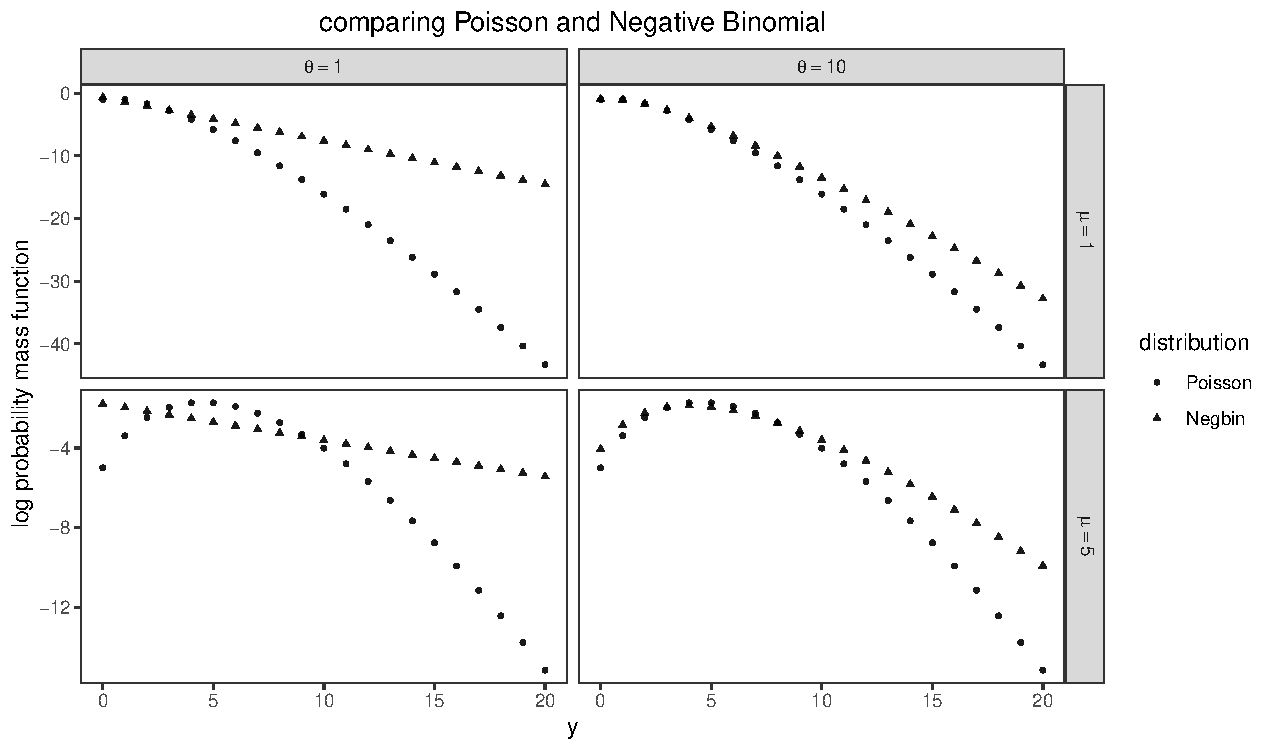
\includegraphics[width = 0.95\textwidth]{figures/poisson_negbin.pdf}
\caption{Comparing the log probabilities of Poisson and Negative-Binomial with the same mean}
\label{fig::poisson-negativebinomial}
\end{figure}



\subsection{Zero-inflated count distributions}

Many count distributions have larger masses at zero compared to Poisson and Negative-Binomial. Therefore, it is also important to have more general distributions capturing this feature of empirical data. We can simply add an additional zero component to the Poisson or the Negative-Binomial. 


A zero-inflated Poisson random variable $y$ is a mixture of two components:
a point mass at zero and a Poisson$(\lambda)$ random variable, with
probabilities $p$ and $1-p$, respectively. So $y$ has the probability
mass function
\[
\pr(y=k)=\begin{cases}
p+(1-p)e^{-\lambda}, & \text{if }k=0,\\
(1-p)e^{-\lambda}\frac{\lambda^{k}}{k!}, & \text{if }k=1,2,\ldots.
\end{cases}
\]
and moments below:
\begin{proposition}
\label{proposition:moments-zeroinflated-poisson}$E(y)=(1-p)\lambda$ and $\var(y)=(1-p)\lambda(1+p\lambda).$
\end{proposition}




A zero-inflated Negative-Binomial random variable $y$ is a mixture
of two components: a point mass at zero and a NB$(\mu,\theta)$ random
variable, with probabilities $p$ and $1-p$, respectively. So $y$
has probability mass function
\[
\pr(y=k)=\begin{cases}
p+(1-p)\left(\frac{\theta}{\mu+\theta}\right)^{\theta}, & \text{if }k=0,\\
(1-p)\frac{\Gamma(k+\theta)}{\Gamma(k+1)\Gamma(\theta)}\left(\frac{\theta}{\mu+\theta}\right)^{\theta}\left(\frac{\mu}{\mu+\theta}\right)^{k}, & \text{if }k=1,2,\ldots.
\end{cases}
\]
and moments below:
\begin{proposition}
\label{proposition:moments-zeroinflated-NB}$E(y)=(1-p)\mu$ and $\var(y)=(1-p) \mu (1+\mu/\theta+p\mu).$
\end{proposition}


I leave the proofs of Propositions \ref{proposition:moments-zeroinflated-poisson} and \ref{proposition:moments-zeroinflated-NB} as Problem \ref{hw19::moment-0-poisson}. 

\section{Regression models for counts}

To model a count outcome $y_{i}$ given $x_{i}$, we can still use
OLS. However, a problem with OLS is that the predicted value can be negative.
This can be easily fixed by running OLS of $\log(y_{i}+1)$ given
$x_{i}$. However, this still does not reflect the fact that $y_{i}$
is a count outcome. For example, these two OLS fits cannot easily make
a prediction for the probabilities $\pr(y_{i}\geq1\mid x_{i})$ or
$\pr(y_{i}>3\mid x_{i})$. A more direct approach is to model the
conditional distribution of $y_{i}$ given $ x_{i}$ using the distributions
reviewed in Section \ref{sec:Some-random-variables-counts}.

\subsection{Poisson regression}

Poisson regression assumes 
\begin{align*}
\begin{cases}
y_{i}  \mid  x_{i} &\sim\text{Poisson}(\lambda_{i}),\\
\lambda_{i} & = \lambda(x_{i},\beta)=e^{x_{i}^{\T}\beta}.
\end{cases}
\end{align*}
So the mean and variance of $y_{i}\mid x_{i}$ are
\[
E(y_{i}\mid x_{i})=\var(y_{i}\mid x_{i})=e^{x_{i}^{\T}\beta}.
\]
Because 
\[
\log E(y_{i}\mid x_{i})=x_{i}^{\T}\beta,
\]
this model is sometimes called the log-linear model, with the coefficient
$\beta_{j}$ interpreted as the conditional log mean ratio:
\[
\log\frac{E(y_{i}\mid  \ldots,x_{ij}+1,\ldots )}{E(y_{i}\mid  \ldots,x_{ij},\ldots )}=\beta_{j}.
\]

The likelihood function for independent Poisson random variables is
\[
L(\beta)=\prod_{i=1}^{n}e^{-\lambda_{i}}\frac{\lambda_{i}^{y_{i}}}{y_{i}!}\propto\prod_{i=1}^{n}e^{-\lambda_{i}}\lambda_{i}^{y_{i}},
\]
and omitting the constants, we can write the log-likelihood function
as
\begin{align*}
\log L(\beta) & =\sumn\left(-\lambda_{i}+y_{i}\log\lambda_{i}\right)=\sumn\left(-e^{x_{i}^{\T}\beta}+y_{i}x_{i}^{\T}\beta\right).
\end{align*}
The score function is
\begin{eqnarray*}
\frac{\partial\log L(\beta)}{\partial\beta} 
&=& \sumn\left(-x_{i}e^{x_{i}^{\T}\beta}+x_{i}y_{i}\right) \\
&=& \sumn x_{i}\left(y_{i}-e^{x_{i}^{\T}\beta}\right) \\
&=&\sumn x_{i}\left\{ y_{i}-\lambda(x_{i},\beta)\right\} ,
\end{eqnarray*}
and the Hessian matrix is
\begin{eqnarray*}
\frac{\partial^{2}\log L(\beta)}{\partial\beta\partial\beta^{\T}} 
& = &-\sumn x_{i}\frac{\partial}{\partial\beta^{\T}}\left(e^{x_{i}^{\T}\beta}\right) \\
&=&-\sumn e^{x_{i}^{\T}\beta}x_{i}x_{i}^{\T}
\end{eqnarray*}
which is negative semi-definite. When the Hessian is negative definite,
the MLE is unique. It must satisfy that
\[
\sumn x_{i}\left(y_{i}-e^{x_{i}^{\T}\hat{\beta}}\right)=\sumn x_{i}\left\{ y_{i}-\lambda(x_{i},\hat{\beta})\right\} =0.
\]
We can solve this nonlinear equation using Newton's method:
\begin{align*}
\beta^{\text{new}} & =\beta^{\text{old}}-\left\{ \frac{\partial^{2}\log L(\beta^{\text{old}})}{\partial\beta\partial\beta^{\T}}\right\} ^{-1}\frac{\partial\log L(\beta^{\text{old}})}{\partial\beta}\\
 & =\beta^{\text{old}}-(X^{\T}W^{\text{old}}X)^{-1}X^{\T}(Y-\Lambda^{\text{old}}),
\end{align*}
where 
\[
X=\left(\begin{array}{c}
x_{1}^{\T}\\
\vdots\\
x_{n}^{\T}
\end{array}\right),\quad Y=\left(\begin{array}{c}
y_{1}\\
\vdots\\
y_{n}
\end{array}\right)
\]
and
\[
\Lambda^{\text{old}}=\left(\begin{array}{c}
\exp(x_{1}^{\T}\beta^{\text{old}})\\
\vdots\\
\exp(x_{n}^{\T}\beta^{\text{old}})
\end{array}\right),\quad W^{\text{old}}=\text{diag}\left\{ \exp(x_{i}^{\T}\beta^{\text{old}})\right\} _{i=1}^{n}.
\]
Similar to the derivation for the logit model, we can simplify Newton's
method to
\[
\beta^{\text{new}}=(X^{\T}W^{\text{old}}X)^{-1}X^{\T}W^{\text{old}}Z^{\text{old}},
\]
where 
\[
Z^{\text{old}}=X\beta^{\text{old}}+(W^{\text{old}})^{-1}(Y-\Lambda^{\text{old}}).
\]
So we have an iterative reweighted least squares algorithm. In \ri{R}, we can use the \ri{glm} function with ``\ri{family = poisson(link = "log")}'' to fit the Poisson regression, which uses Newton's method. 
 

Statistical inference based on 
\[
\hat{\beta}\asim\N\left\{ \beta,\left(-\frac{\partial^{2}\log L(\hat{\beta})}{\partial\beta\partial\beta^{\T}}\right)^{-1}\right\} =\N\left\{ \beta,(X^{\T}\hat{W}X)^{-1}\right\} ,
\]
where $\hat{W}=\text{diag}\left\{ \exp(x_{i}^{\T}\hat{\beta})\right\} _{i=1}^{n}$. 


After obtaining the MLE, we can predict the mean $E(y_i \mid x_i)$ by $ \hat{\lambda}_i =  e^{x_i^{\T} \hat{\beta}} $. Because Poisson regression is a fully parametrized model, we can also predict any other probability quantities involving $y_i \mid x_i$. For example, we can predict  $\pr(y_i = 0  \mid x_i)$ by $e^{- \hat{\lambda}_i }$, and $\pr(y_i \geq 3 \mid x_i) $ by $1 - e^{- \hat{\lambda}_i } (1 + \hat{\lambda}_i  + \hat{\lambda}_i ^2/2 )$. 




\subsection{Negative-Binomial regression}

Negative-Binomial regression assumes 
\begin{align*}
\begin{cases}
y_{i}  \mid x_{i} &\sim\text{NB}(\mu_{i},\theta),\\
\mu_{i} & =e^{x_{i}^{\T}\beta},
\end{cases}
\end{align*}
so it has conditional mean and variance:
$$
E (y_{i}  \mid x_{i} ) = e^{x_{i}^{\T}\beta} ,\quad 
\var (y_{i}  \mid x_{i} ) = e^{x_{i}^{\T}\beta} (1+e^{x_{i}^{\T}\beta} / \theta) . 
$$
It is also a log-linear model. 

The log-likelihood function for Negative-Binomial regression is $\log L(\beta, \theta) = \sumn l_i(\beta, \theta)$ with
\begin{eqnarray*}
 l_i(\beta, \theta)  
&=&     \log \Gamma(y_i+\theta) - \log \Gamma(y_i + 1) - \log \Gamma(\theta)    \\
 && + \theta\log \left( \frac{\theta}{\mu_i +\theta} \right) + y_i \log \left( \frac{ \mu_i  }{ \mu_i  + \theta} \right) , 
\end{eqnarray*}
where $\mu_i  = e^{x_{i}^{\T}\beta}$ has partial derivative $\partial \mu_i / \partial \beta = \mu_i x_i$. 
We can use Newton's algorithm or Fisher scoring algorithm to compute the MLE $(\hat\beta, \hat\theta)$ which requires deriving the first and second derivatives of $\log L(\beta, \theta)$ with respect to $(\beta, \theta)$. I will derive some important components and relegate other details to Problem \ref{hw19::derivatives-nb-reg}. First,
$$
\frac{ \partial \log L(\beta, \theta) }{\partial \beta} =
\sumn  (1+ \mu_i/\theta )^{-1} (y_i - \mu_i) x_i. 
$$
The corresponding first-order condition can be viewed as the estimating equation of Poisson regression with weights $  (1+ \mu_i/\theta )^{-1}$. Second,
$$
\frac{ \partial ^2 \log L(\beta, \theta) }{\partial \beta \partial \theta}
= \sumn  \frac{  \mu_i   }{  (\mu_i + \theta)^2  } (y_i - \mu_i) x_i.
$$
We can verify
$$
E\left\{ \frac{ \partial ^2 \log L(\beta, \theta) }{\partial \beta \partial \theta}  \mid X \right\} = 0
$$
since each term inside the summation has conditional expectation zero. This implies that the Fisher information matrix is diagonal, so $\hat\beta$ and $ \hat\theta$ are asymptotically independent. 

The \ri{glm.nb} in the \ri{MASS} package iterate between $\beta$ and $\theta$: given $\theta$, update $\beta$ based on Fisher scoring; given $\beta$, update $\theta$ based on Newton's algorithm. It reports standard errors based on the inverse of the Fisher information matrix.\footnote{
The command \texttt{rnbreg}   in \texttt{Stata} uses the Berndt--Hall--Hall--Hausman (BHHH) algorithm by default, which may give slightly different numbers compared with \texttt{R}. The BHHH algorithm is similar to Newton's algorithm but avoids calculating the Hessian matrix. 
}
 

\subsection{Zero-inflated regressions}

The zero-inflated Poisson regression assumes that 
\[
y_{i}\mid x_{i}\sim\begin{cases}
0, & \text{with probability }p_{i},\\
\text{Poisson}(\lambda_{i}), & \text{with probability }1-p_{i},
\end{cases}
\]
where 
$$
p_{i}  =\frac{e^{x_{i}^{\T}\gamma}}{1+e^{x_{i}^{\T}\gamma}},\quad 
\lambda_{i}  = e^{x_{i}^{\T}\beta}.
$$

 
The zero-inflated Negative-Binomial regression assumes that
\[
y_{i}\mid x_{i}\sim\begin{cases}
0, & \text{with probability }p_{i},\\
\text{NB}(\mu_{i},\theta), & \text{with probability }1-p_{i},
\end{cases}
\]
where 
$$
p_{i}  =\frac{e^{x_{i}^{\T}\gamma}}{1+e^{x_{i}^{\T}\gamma}},\quad 
\mu_{i}  = e^{x_{i}^{\T}\beta} .
$$

To avoid over-parametrization, we can also restrict some coefficients
to be zero. 
The  \ri{zeroinfl} function in the \ri{R} package \ri{pscl} can fit the zero-inflated Poisson and Negative-Binomial regressions. 


\section{A case study}\label{sec::count-case-study}

I will use the dataset from \citet{royer2015incentives} to illustrate the regressions for count outcomes. The \ri{R} code is in \ri{code21.3.R}. 
From the regression formula below, we are interested in the effect of two treatments \ri{incentive_commit} and \ri{incentive} on the number of visits to the gym, controlling for two pretreatment covariates \ri{target} and \ri{member_gym_pre}. 

\begin{lstlisting}
> library("foreign")
> library("MASS")
> gym1 = read.dta("gym_treatment_exp_weekly.dta")
> f.reg = weekly_visit ~ incentive_commit + incentive + 
+   target + member_gym_pre
\end{lstlisting}



\subsection{Linear, Poisson, and Negative-Binomial regressions}

\begin{figure}[ht]
\centering
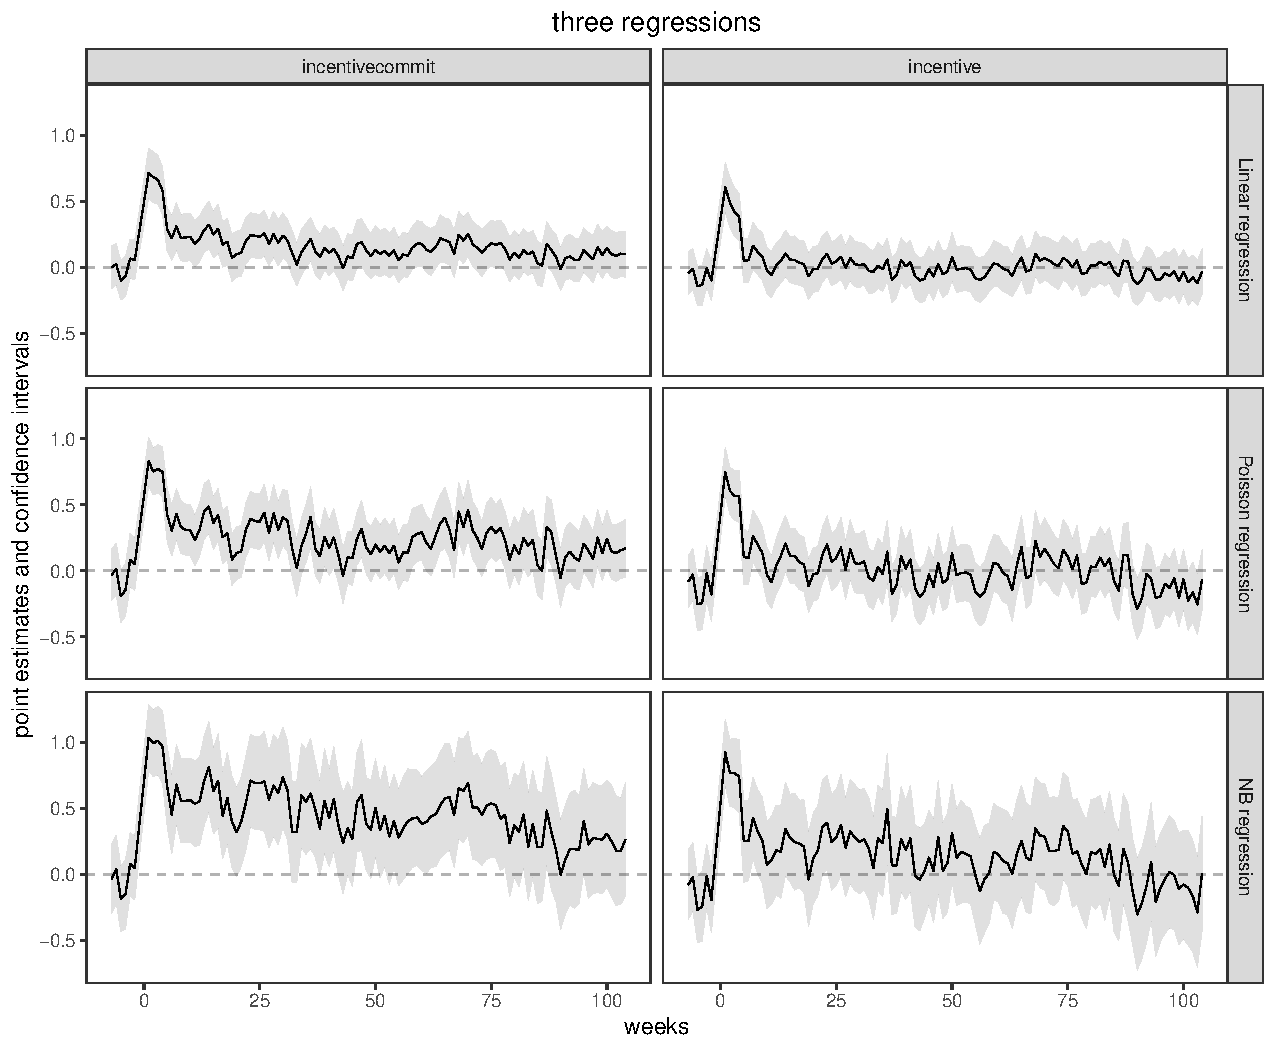
\includegraphics[width = 0.95\textwidth]{figures/threeregressions.pdf}
\caption{Linear, Poisson, and Negative-Binomial regressions}\label{fig::three regressions}
\end{figure}



Each worker was observed over time, so we run regressions with the outcome data observed in each week. In the following, we compute the linear regression coefficients, standard errors, and AICs. 

\begin{lstlisting}
> weekids             = sort(unique(gym1$incentive_week))
> lweekids            = length(weekids)
> coefincentivecommit = 1:lweekids
> coefincentive       = 1:lweekids
> seincentivecommit   = 1:lweekids
> seincentive         = 1:lweekids
> AIClm               = 1:lweekids
> for(i in 1:lweekids)
+ {
+         gymweek = gym1[which(gym1$incentive_week == weekids[i]), ]   
+         regweek = lm(f.reg, data = gymweek)
+         regweekcoef = summary(regweek)$coef
+         
+         coefincentivecommit[i] = regweekcoef[2, 1]
+         coefincentive[i]       = regweekcoef[3, 1]
+         seincentivecommit[i]   = regweekcoef[2, 2]
+         seincentive[i]         = regweekcoef[3, 2]
+         
+         AIClm[i]               = AIC(regweek)
+ }
\end{lstlisting}


By changing the line with \ri{lm} by 
\begin{lstlisting}
regweek = glm(f.reg, family = poisson(link = "log"), data = gymweek)
\end{lstlisting}
and 
\begin{lstlisting}
regweek = glm.nb(f.reg, data = gymweek)
\end{lstlisting}
we obtain the corresponding results from Poisson and Negative-Binomial regressions. Figure \ref{fig::three regressions} compares the regression coefficients with the associated confidence intervals over time. Three regressions give very similar patterns: \ri{incentive_commit} has both short-term and long-term effects, but \ri{incentive} only has short-term effects.  



The left panel of Figure \ref{fig::overdispersion-gym} shows that variances are larger than the means for outcomes from all weeks, and the right panel of Figure \ref{fig::overdispersion-gym} shows the point estimates and confidence intervals of $\theta$ from Negative-Binomial regressions. Overall, overdispersion seems an important feature of the data. 


\begin{figure}
\centering
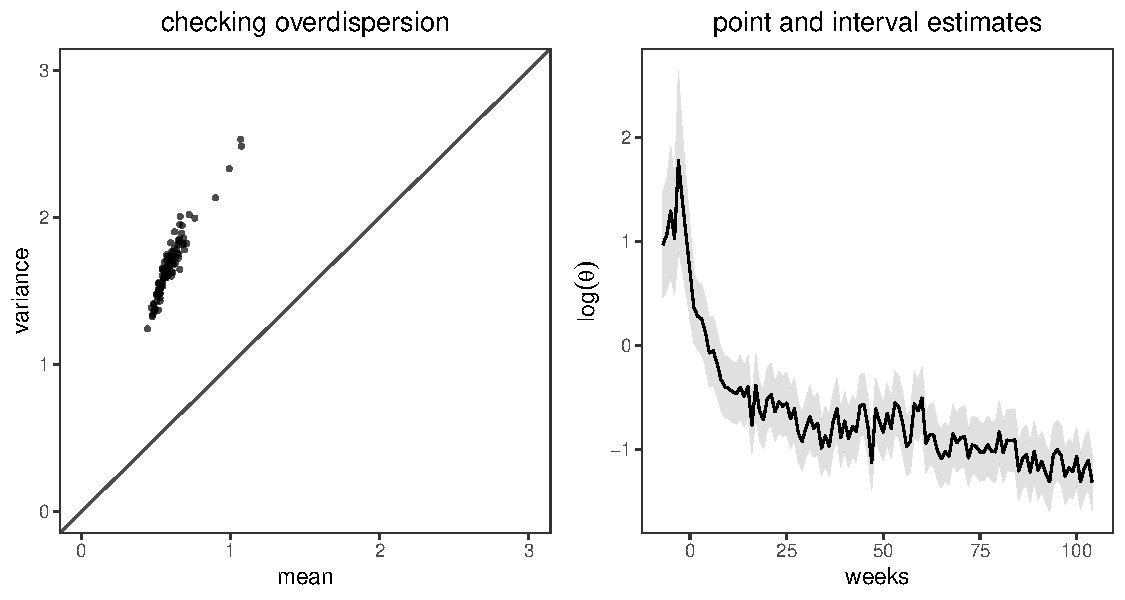
\includegraphics[width = 0.8\textwidth]{figures/gym_overdispersion_check.pdf}
\caption{Overdispersion of the data}\label{fig::overdispersion-gym}
\end{figure}



\subsection{Zero-inflated regressions}


Figure \ref{fig::zeroinflation-gym} plots the histograms of the outcomes from four weeks before and four weeks after the experiment. Eight histograms all show severe zero inflation because most workers just did not go to the gym regardless of the treatments. Therefore, it seems crucial to accommodate the zeros in the models. 

\begin{figure}[ht]
\centering
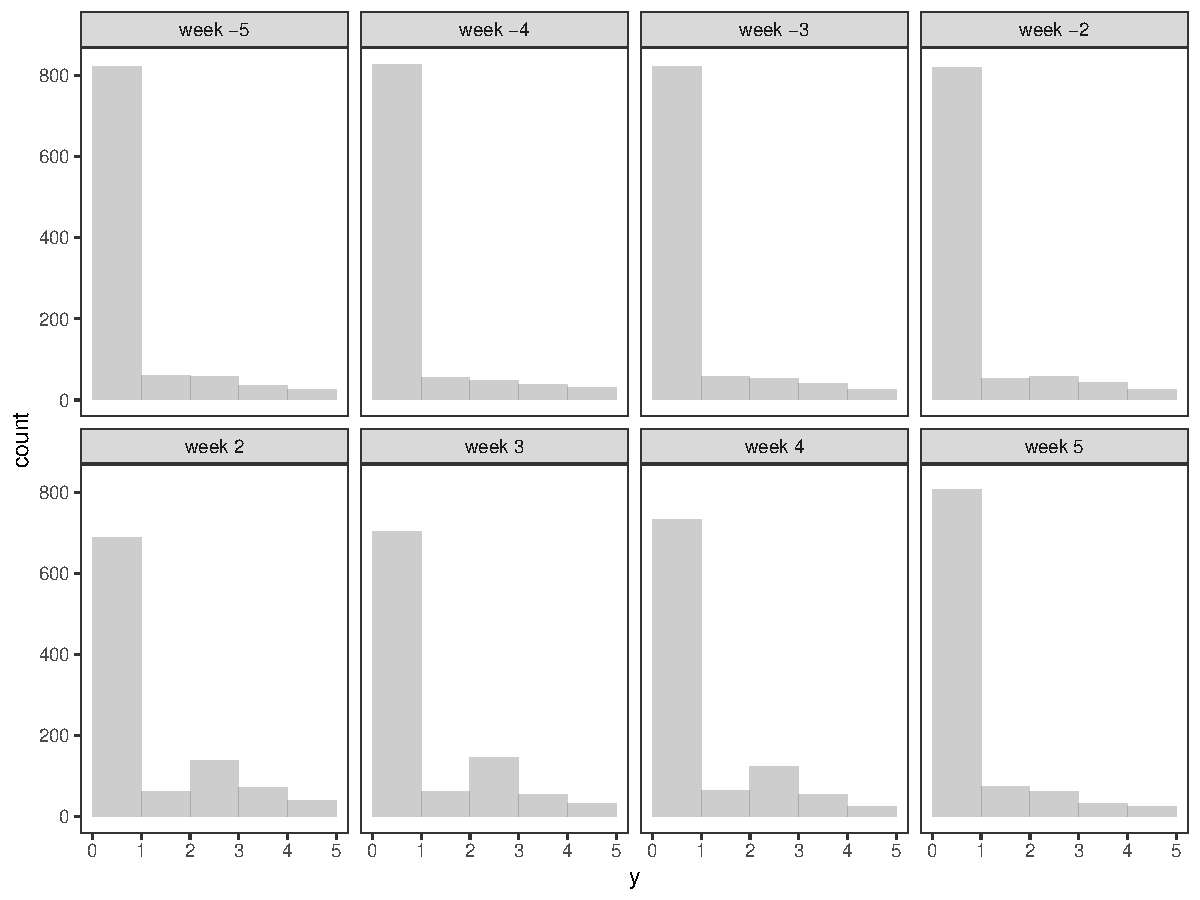
\includegraphics[width = 0.8\textwidth]{figures/gym_check_zeroinf.pdf}
\caption{Zero-inflation of the data}\label{fig::zeroinflation-gym}
\end{figure}


\begin{figure}[ht]
\centering
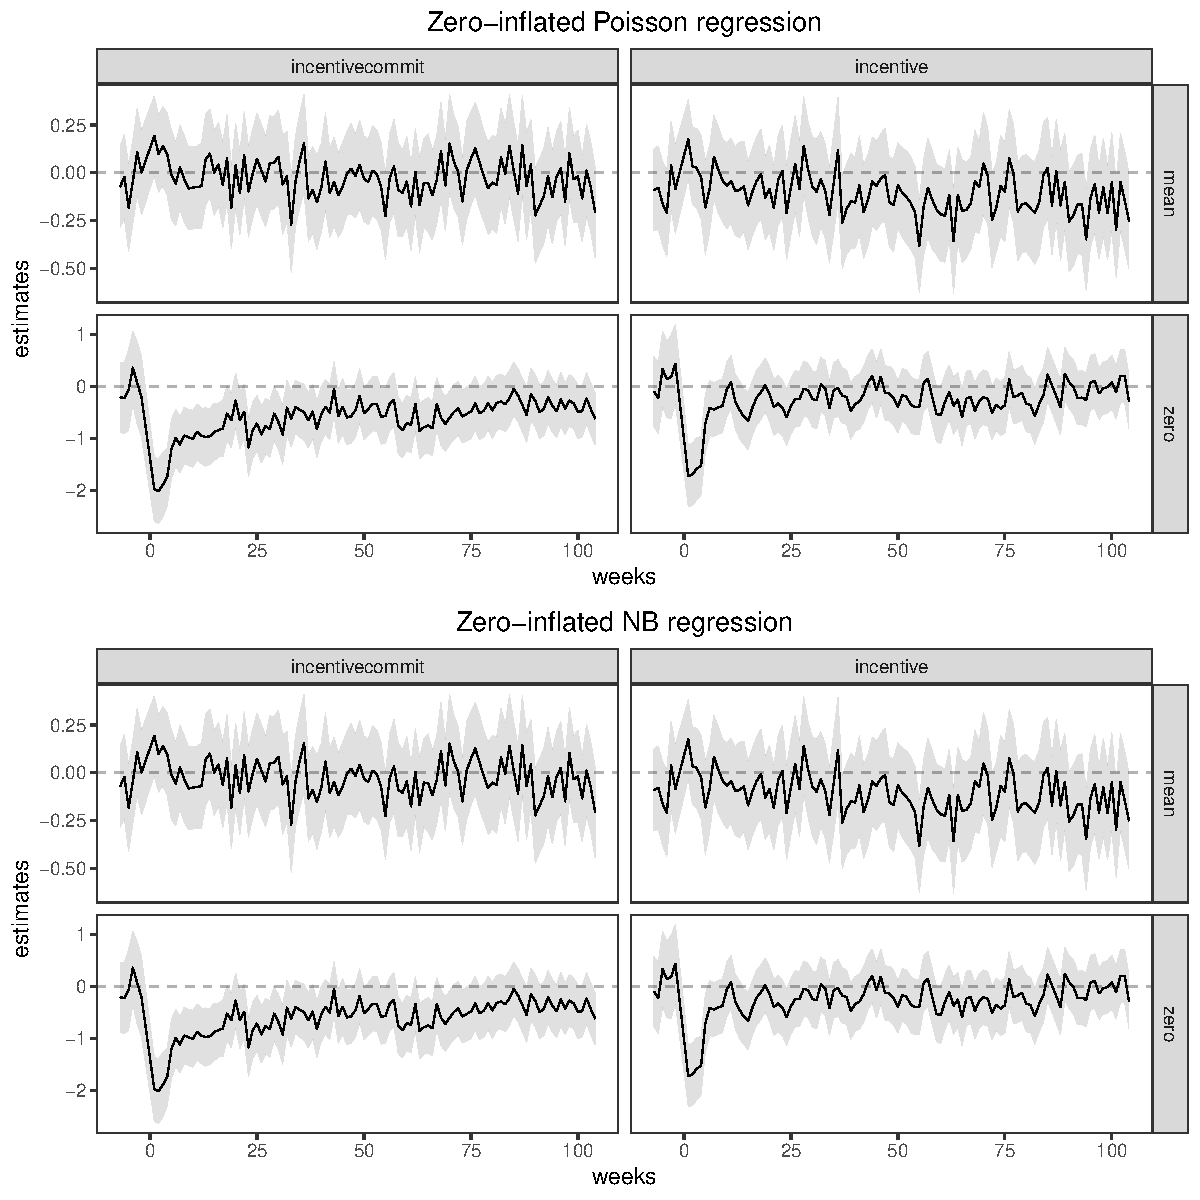
\includegraphics[width = 0.95\textwidth]{figures/gym_zeroinflated_regressions.pdf}
\caption{Zero-inflated regressions}\label{fig::zeroinflated-regressions-gym}
\end{figure}

We now fit zero-inflated Poisson regressions. The model has parameters for the zero component and parameters for the Poisson components. 

\begin{lstlisting}
> library("pscl")
> coefincentivecommit0 = coefincentivecommit
> coefincentive0       = coefincentive
> seincentivecommit0   = seincentivecommit
> seincentive0         = seincentive
> AIC0poisson          = AICnb
> for(i in 1:lweekids)
+ {
+   gymweek = gym1[which(gym1$incentive_week == weekids[i]), ]   
+   regweek = zeroinfl(f.reg, dist = "poisson", data = gymweek)
+   regweekcoef = summary(regweek)$coef
+   
+   coefincentivecommit[i] = regweekcoef$count[2, 1]
+   coefincentive[i]       = regweekcoef$count[3, 1]
+   seincentivecommit[i]   = regweekcoef$count[2, 2]
+   seincentive[i]         = regweekcoef$count[3, 2]
+   
+   coefincentivecommit0[i] = regweekcoef$zero[2, 1]
+   coefincentive0[i]       = regweekcoef$zero[3, 1]
+   seincentivecommit0[i]   = regweekcoef$zero[2, 2]
+   seincentive0[i]         = regweekcoef$zero[3, 2]
+   
+   AIC0poisson[i]          = AIC(regweek)
+ }
\end{lstlisting}

Replacing the line with \ri{zeroinfl} by 
\begin{lstlisting}
  regweek = zeroinfl(f.reg, dist = "negbin", data = gymweek)
\end{lstlisting}
we can fit the corresponding zero-inflated Negative-Binomial regressions. Figure \ref{fig::zeroinflated-regressions-gym} plots the point estimates and the confidence intervals of the coefficients of the treatment. It shows that the treatments do not have effects on the Poisson or Negative-Binomial components, but have effects on the zero components. This suggests that the treatments affect the outcome mainly by changing the workers' behavior of whether to go to the gym. 




Another interesting result is the large $\hat{\theta}$'s from the zero-inflated Negative-Binomial regression:
\begin{lstlisting}
> quantile(gymtheta, probs = c(0.01, 0.25, 0.5, 0.75, 0.99))
  1%  25%  50%  75%  99% 
12.3 13.1 13.7 14.4 15.7 
\end{lstlisting}


Once the zero-inflated feature has been modeled, it is not crucial to account for the overdispersion. It is reasonable because the maximum outcome is five, ruling out heavy-tailedness. This is further corroborated by the following comparison of the AICs from five regression models. Figure \ref{fig::comparing-aic-gym} shows that zero-inflated Poisson regressions have the smallest AICs, beating the zero-inflated Negative-Binomial regressions, which are more flexible but have more parameters to estimate. 

\begin{figure}[ht]
\centering
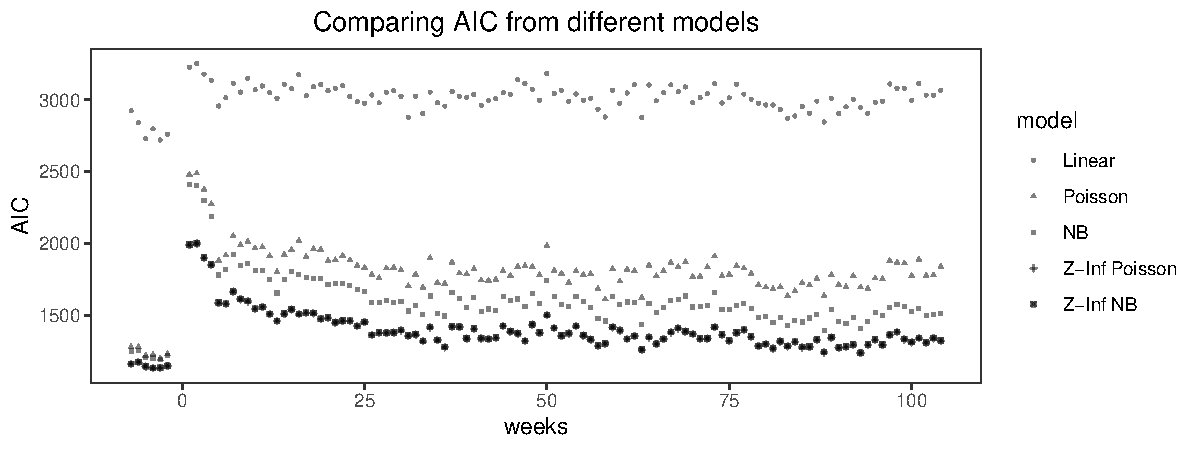
\includegraphics[width = \textwidth]{figures/gym_comparing_aic.pdf}
\caption{Comparing AICs from five regression models}\label{fig::comparing-aic-gym}
\end{figure}





\section{Homework problems}

 

\paragraph{Newton's method for Negative-Binomial regression}\label{hw19::derivatives-nb-reg}

Calculate the score function and Hessian matrix based on the log-likelihood function of the Negative-Binomial regression.
What is the joint asymptotic distribution of the MLE $(\hat\beta, \hat\theta)$?





\paragraph{Moments of Zero-inflated Poisson and Negative-Binomial}\label{hw19::moment-0-poisson}

Prove Propositions \ref{proposition:moments-zeroinflated-poisson} and \ref{proposition:moments-zeroinflated-NB}. 


\paragraph{Overdispersion and zero-inflation}

Show that for a zero-inflated Poisson, if $p \leq 1/2$ then $E(y) < \var(y)$ always holds. What is the condition for $E(y) < \var(y)$ when $p>1/2$?




\paragraph{Poisson latent variable and the binary regression model with the cloglog link}\label{hw19::poisson-logistic}

Assume that $y_{i}^* \mid x_{i}\sim\text{Poisson}(e^{x_{i}^{\T}\beta})$,
and define $y_{i}=1(y_{i}^*>0)$ as the indicator that $y_{i}^*$ is
not zero. Show that $y_{i} \mid x_{i}$ follows a cloglog model, that
is,
\[
\pr(y_{i} =1\mid x_{i})=g(x_{i}^{\T}\beta),
\]
where $g(z)=1-\exp(-e^{z})$. 

Remark: The cloglog model for binary outcome arises naturally from a latent Poisson model. It was only briefly mentioned in Chapter \ref{chapter::binary-logit}. 



\paragraph{Likelihood for the zero-inflated Poisson regression}

Write down the likelihood function for the Zero-inflated Poisson model,
and derive the steps for Newton's method. 

\paragraph{Likelihood for the Zero-inflated Negative-Binomial regression}

Write down the likelihood function for the Zero-inflated Negative-Binomial model, and
derive the steps for Newton's method. 


\paragraph{Prediction in the Zero-inflated Negative-Binomial regression}

After obtaining the MLE $(\hat{\beta}, \hat{\gamma})$ and its asymptotic covariance matrix $\hat{V}$, predict the conditional mean $E(y_i \mid x_i)$, the conditional probability $\pr(y_i=0\mid x_i)$, and the conditional probability $\pr(y_i \geq 5\mid x_i)$. What are the associated asymptotic standard errors? 


\paragraph{Data analysis}

\citet{zeileis2008regression} gives a tutorial on count outcome regressions using the dataset from \citet{deb1997demand}. Replicate and extend their analysis based on the discussion in this chapter. 
 
 
\paragraph{Data analysis} 


\citet{fisman2007corruption} was an application of Negative-Binomial regression, and \citet{albergaria2017narrow} replicated their study and argued that the zero-inflated Negative-Binomial regression was more appropriate. Replicate and extend their analysis based on the discussion in this chapter. 
